%Struktur
% -Festlegung von Software-Kriterien
% -Auswahl des Verfahrens
% -Reproduktion des Verfahrens aus der Literatur
% 	-Kantenerkennung
% 	-Segmentierung
%	-Probleme & besondere Erkenntnisse
% -Erweiterung des Verfahrens
%	-Grundlegende Änderungen des Verfahrens
%	-False edge removal
%	-Point marking and cloud filtering
%	-misc.


\chapter{Entwicklungsprozess der Software}
Die Rücksichtnahme des Einsatzzwecks bei der Design und Entwurf des Verfahrens sowie die Entwicklung der Software war erforderlich, um die gewünschte Funktionalitäten gewährleisten zu können. Das Verfahren soll Kanten und Geometrien nicht nur in vollständig generierten Punktwolken erkennen, sondern auch in unvollständige Punktwolken, die iterativ wachsen. Hierbei wird ein Laserliniensensor eine Kante eines Werkstücks oder Objektes entlang geführt und somit sequentiell abgetastet. Deswegen wird die räumliche Struktur des Objektes nicht in einer einzigen Aufnahme abgebildet, sondern durch mehrere kleine Einzelaufnahmen. Der intelligente Schweißroboter, der durch das Fraunhofer Institut für Produktions- und Automatisierungstechnik entwickelt wird, verwendet ein solches Verfahren zum Scannen eines Werkstückes und zur Erkennung Schweißnähte \autocite[39]{savla_intelligente_2022}. Mittels eines Lasersensors wird die Oberfläche des Werkstückes dreidimensional abgebildet. Aktuell wird eine Schweißkegelnaht durch die Erkennung der Schnittlinie zwei Ebenen markiert, die mittels RANSAC-Algorithmen auf die Punktwolke des Werkstückes gefittet werden. Dieses Verfahren zur Erkennung der Schweißnaht bietet allerdings kaum detaillierte Informationen über die Geometrie des Werkstückes an.\autocite[39-52]{savla_intelligente_2022}. Das, in dieser Arbeit entwickelte Verfahren soll das bestehende Verfahren ersetzen und somit seine Limitationen überwinden.

\begin{figure}[h]
	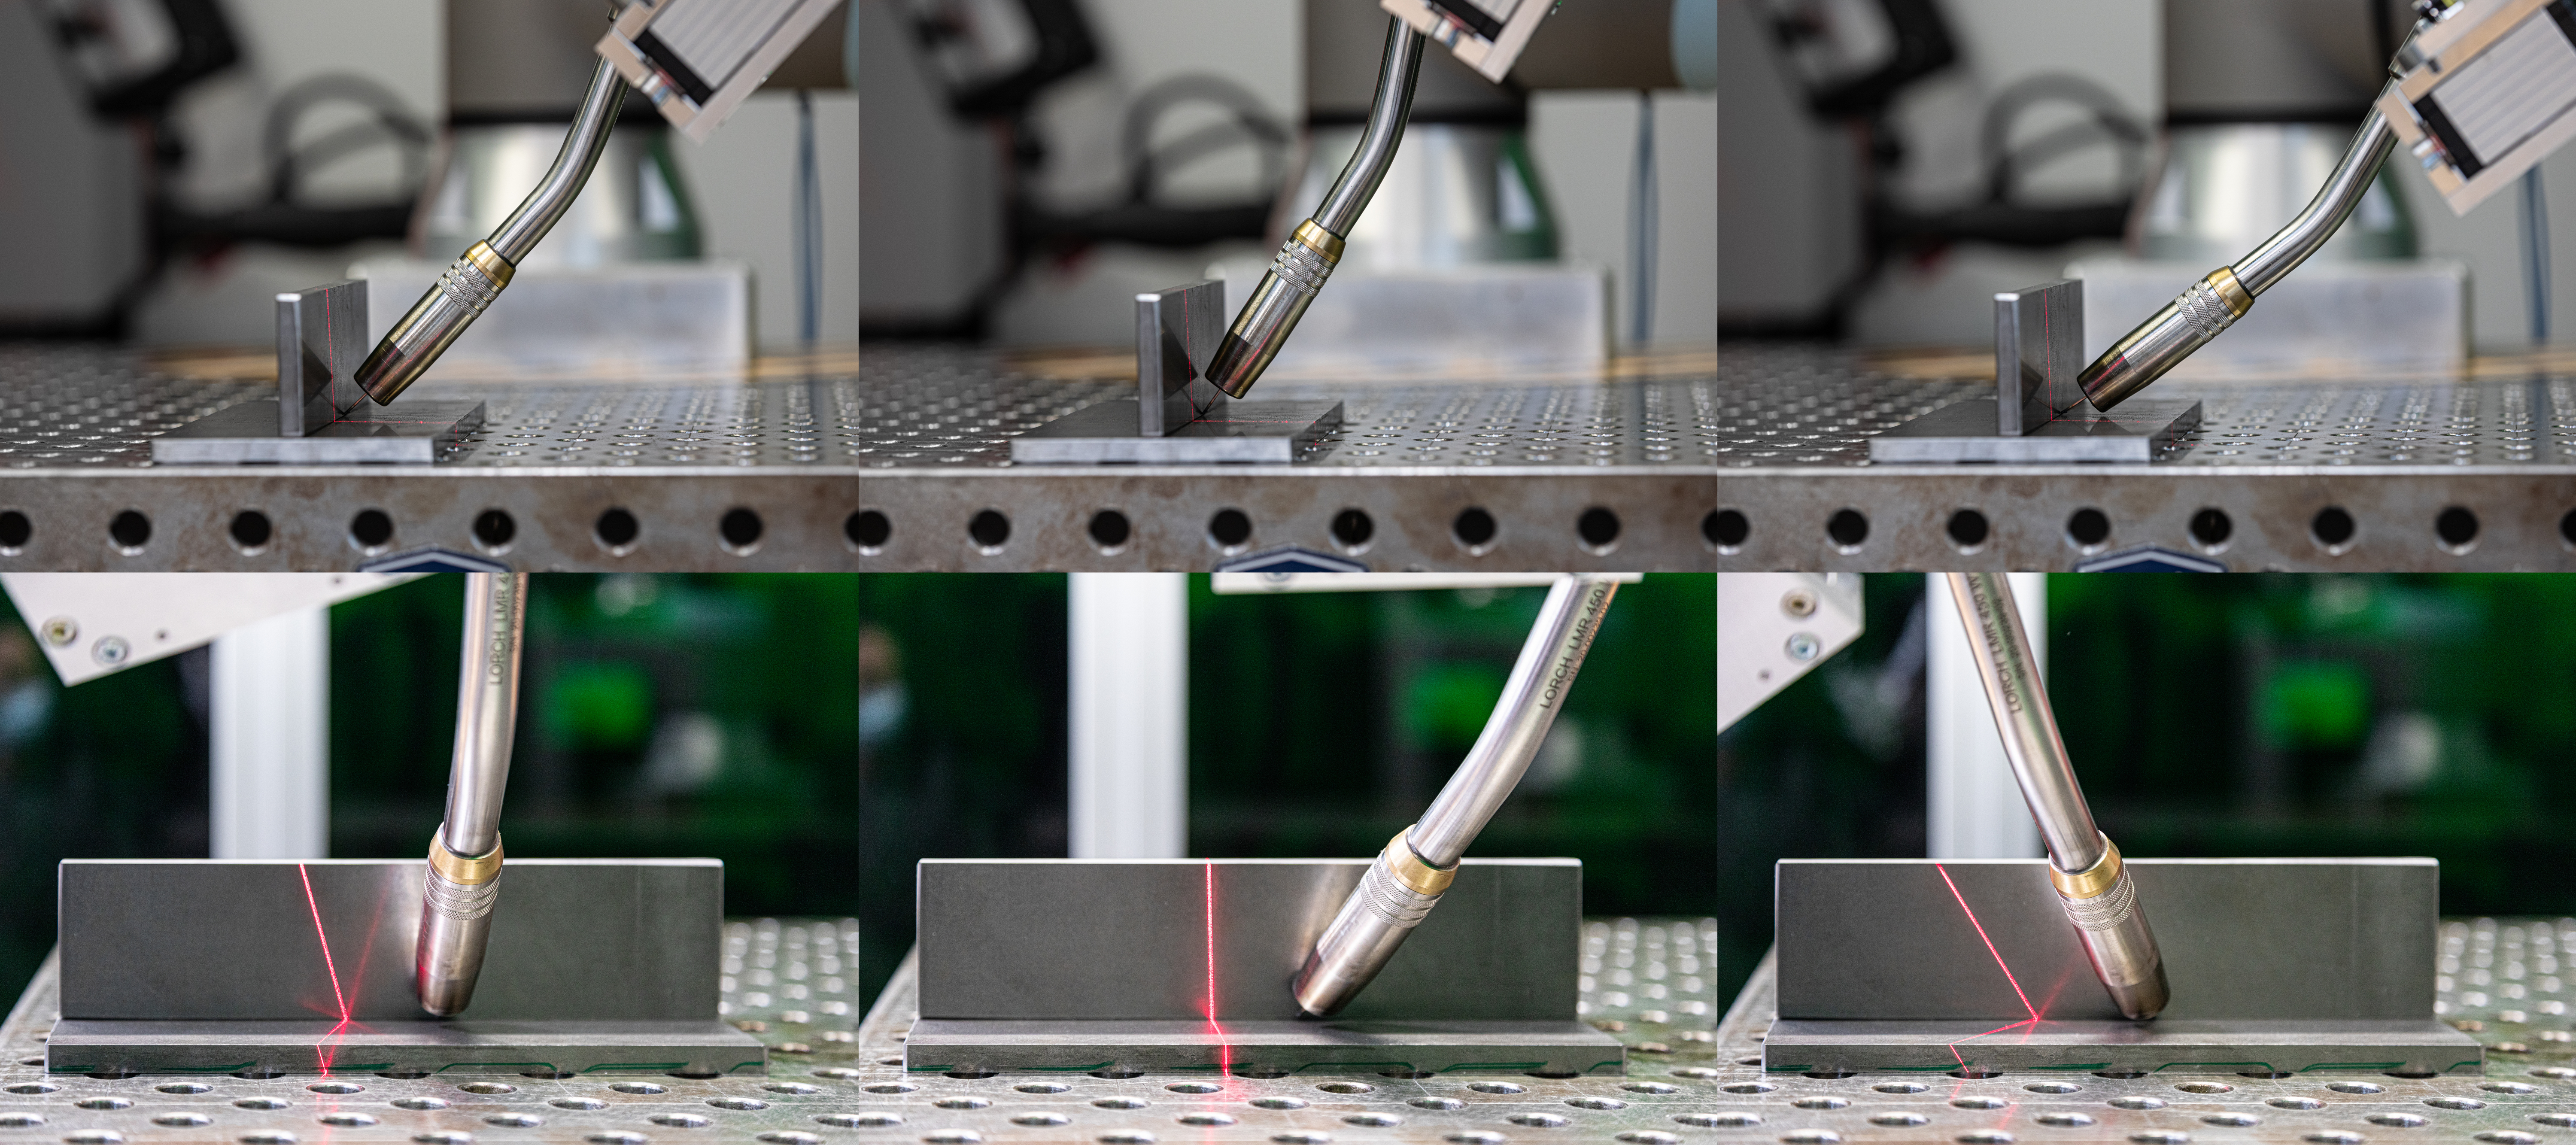
\includegraphics[width = \textwidth]{Abbildungen/collage.jpg}
	\centering
	\caption{Der Laserliniensensor} 
\end{figure}

\section{Vorbereitungen}
\subsection{Software-Voraussetzungen}\label{soft_voraus}
Bei der Auswahl eines geeigneten Verfahrens zur Detektierung Kanten in einer Punktwolke wurden einige Voraussetzungen festgelegt. Die Methode sollte in der Lage sein, nicht nur Außenkanten zu erkennen, sondern auch Innenkanten beziehungsweise Faltungen. Neben dem originellen Einsatzzweck sollte das Verfahren möglichst breit anwendbar sein und eine hohe Modularität aufweisen. Die Funktionen der Kantendetektierung und Punktesegmentierung sollten unabhängig von einander aufrufbar gestaltet werden, um dem Benutzer eine möglichst hohe Flexibilität anzubieten. Die Kantenerkennung sollte performant erfolgen und Punktwolken innerhalb eines praktischen Zeitraums verarbeiten. Letztlich soll das Programm in dem bestehenden Programmpaket des Schweißroboters integrierbar sein. Die Hardwarebeschleunigung des Verfahrens mittels eines Grafikprozessors wurde ausgeschlossen, da ihrer Verwendung mit dem Echtzeitkernels des Programmpakets zur Konflikte führt. 

\subsection{Auswahl eines Verfahrens}
Eine Literatursuche nach Verfahren zur adaptiven Erkennung von Kanten in wachsenden 3D Punktwolken für den Einsatzzweck ergab nichts. Die meisten Verfahren eigneten sich für die Kantenerkennung nur in vollständigen Punktwolken. Aus diesem Grund wurde die Entscheidung getroffen, ein vorhandenes Verfahren aus der Literatur zu wählen und es für den Einsatzzweck anzupassen. Drei unterschiedlichen Verfahren nach \textcite{bazazian_edc-net_2021}, \textcite{himeur_pcednet_2021} und \textcite{rachmadi_road_2017} zeigten viel versprechende Ergebnisse. Allerdings wurden neuronale Netze in dieser Verfahren verwendet, welches zu zwei Problemen geführt hätte. Aufgrund der Funktionsweise neuronaler Netze wäre es schwierig gewesen, diese für den Einsatzzweck ohne eine umständliche Anpassung des neuronalen Netzes anzupassen. Das zweite Hindernis entsteht durch die Einschränkung bei der Verwendung von Grafikprozessoren. Diese Prozessoren hätten die Rechenzeit neuronaler Netze sehr stark verringert und die schnelle Performanz des Verfahrens gewährleistet \autocite[625]{luo_artificial_2005}. Das numerische Verfahren nach \textcite{choi_rgb-d_2013} war auch für den Einsatzzweck ungeeignet, da es als Eingangsparameter eine RGB-D Datei erfordert. Somit wäre das Verfahren nur für eine Anwendung auf organisierten, gefärbten Punktwolken eingeschränkt. Es wurden zwei weitere Verfahren gefunden, die sich zur Erkennung Kanten in organisierten sowie unorganisierten Punktwolken eignen würden. \textcite{mineo_novel_2019} stellten eine numerische Methoden vor, welche zu einer hohen Genauigkeit Kanten erkennen konnte. Allerdings wurden keine Angaben über die Erkennung Innenkanten in dieser Arbeit gemacht. \textcite{ni_edge_2016} schlagen im Gegensatz eine Methode namens AGPN vor, die nicht nur Außen- sowie Innenkanten und Faltungen erkennt, sondern die erkannten Randpunkte zusammen clustert, um Kannten voneinander zu trennen. Diese Studie präsentierte ein Verfahren mit einer hohen Genauigkeit sowie eine Möglichkeit, die Randpunkte sinnvoll zusammen zu gruppieren. Aus diesem Grund wurde dieses Verfahren als Grundlage für das adaptive Verfahren dieser Arbeit gewählt.

\section{Reproduktion des AGPNs}
Bevor das Verfahren für den Einsatzzweck angepasst wurde, wurde es zuerst zwecks einer Überprüfung unverändert implementiert. Es sollte sichergestellt werden, dass das Verfahren für die Erkennung Innenkanten und potenzielle Schweißnähte geeignet ist. Da die Autoren das Quellcode ihres Verfahrens nicht öffentlich zugängig gemacht haben, musste das Programm händisch reproduziert werden. Die Reproduktion des Programms erfolgte in zwei Schritten - die Reproduktion des Verfahrens zur Kantenerkennung und dessen zur Kantensegmentierung. Obwohl andere Skriptsprachen wie Python und MATLAB hinsichtlich des Prototypings Vorteile anbieten, wurde das Programm in C++ wegen seiner besseren Leistungsfähigkeit implementiert \autocite{svensson_performance_2021}. Viele Funktionalitäten der PCL-Bibliothek wurden für dieses Verfahren verwendet.
%TODO: reference PCL 

\subsection{Verfahren zur Erkennung Randpunkte}
Während Randelemente in zweidimensionale Bilder als eine klare Definition haben, fehlt eine solche Definition für Randelemente und Kanten in 3D-Punktwolken. In diesem Verfahren wurden die geometrischen Eigenschaften einer Kollektion von Punkten zur Erkennung Randpunkte berücksichtigt. Randpunkte weisen eine besondere geometrische Eigenschaft auf - der Winkelabstand zwischen benachbarten Randpunkte ist im Vergleich zu anderen benachbarten Punkten deutlich größer. Faltungen stellen den Grenzbereich zwischen zwei angrenzenden Ebenen dar, deren Normale in unterschiedlichen Richtungen zeigen. Diese geometrischen Eigenschaften wurden zur Erkennung Randpunkte verwendet. \autocite[1-2]{ni_edge_2016}

Im folgenden wird das Verfahren zur Erkennung Randpunkte detaillierter erläutert. Für einen Punkt \textit{o} wurde eine Sammlung \textit{P\textsubscript{o}} von \textit{K} benachbarten Punkten mittels eines kd-trees erstellt. Diese Sammlung wird als eine Nachbarschaft referiert. 